\documentclass{report}

\usepackage{float}
\usepackage{titlesec}
\usepackage{graphicx}
\usepackage{amsmath}
\usepackage{subcaption}
\usepackage{listings}
\usepackage{xcolor}

\graphicspath{ {./assets/} {..} }

\newcommand{\subimgw}{.5\linewidth}

\definecolor{codegreen}{rgb}{0,0.6,0}
\definecolor{codegray}{rgb}{0.5,0.5,0.5}
\definecolor{codepurple}{rgb}{0.58,0,0.82}
\definecolor{backcolour}{rgb}{0.95,0.95,0.92}

\lstdefinestyle{mys}{
    backgroundcolor=\color{backcolour},   
    commentstyle=\color{codegreen},
    keywordstyle=\color{magenta},
    numberstyle=\tiny\color{codegray},
    stringstyle=\color{codepurple},
    basicstyle=\ttfamily\footnotesize,
    breakatwhitespace=false,
    breaklines=true,
    captionpos=b,
    keepspaces=true,
    numbers=left,
    numbersep=5px,
    showspaces=false,
    showstringspaces=false,
    showtabs=false,
    tabsize=2
}
\lstset{style=mys}

\author{
  Kristian Henrik Salen Sørli
  \and
  William B. Sørensen\\
}
\title{TOF Rapport}
\begin{document}
\maketitle

\tableofcontents

\chapter{Oppgaver}

\addcontentsline{toc}{section}{Oppgave 1}
\section*{Oppgave 1}

\subsection*{A}

I denne oppgaven ble det laget en rekke figurer ut av spagettis. Grunnen til dette var for å se hvordan effekt forskyvings kreftene hadde på de forskjellige figurene med å se hvilken av sidene knakk når figuren ble underlagt trykk.

Fra et polygonalt perspektiv er den mest uniformt integral figuren en likesidet trekant. Dette kommer av at den tåler like mye trekk og forskyvning krefter fra hver side av figuren gjennom at den fordeler krafta likt.

En likebeint trekant er sterkest på den korteste siden. Grunnen til dette er siden forskyvnings-kraften blir fordelt over de to lengere sidene.

En rettvinklet trekant er sterkest på den korteste katen.

En firkant er svakest siden den har mulighet til å oppleve plan-forskyvning.

\subsection*{B}

Triangulær pyramide har de samme styrkene som en likesidet trekant hvor hvor den tåler fra hver av sidene og den fordeler likt gjennom hele figuren

\begin{figure}[H]
	\begin{subfigure}{.5\textwidth}
		\centering
		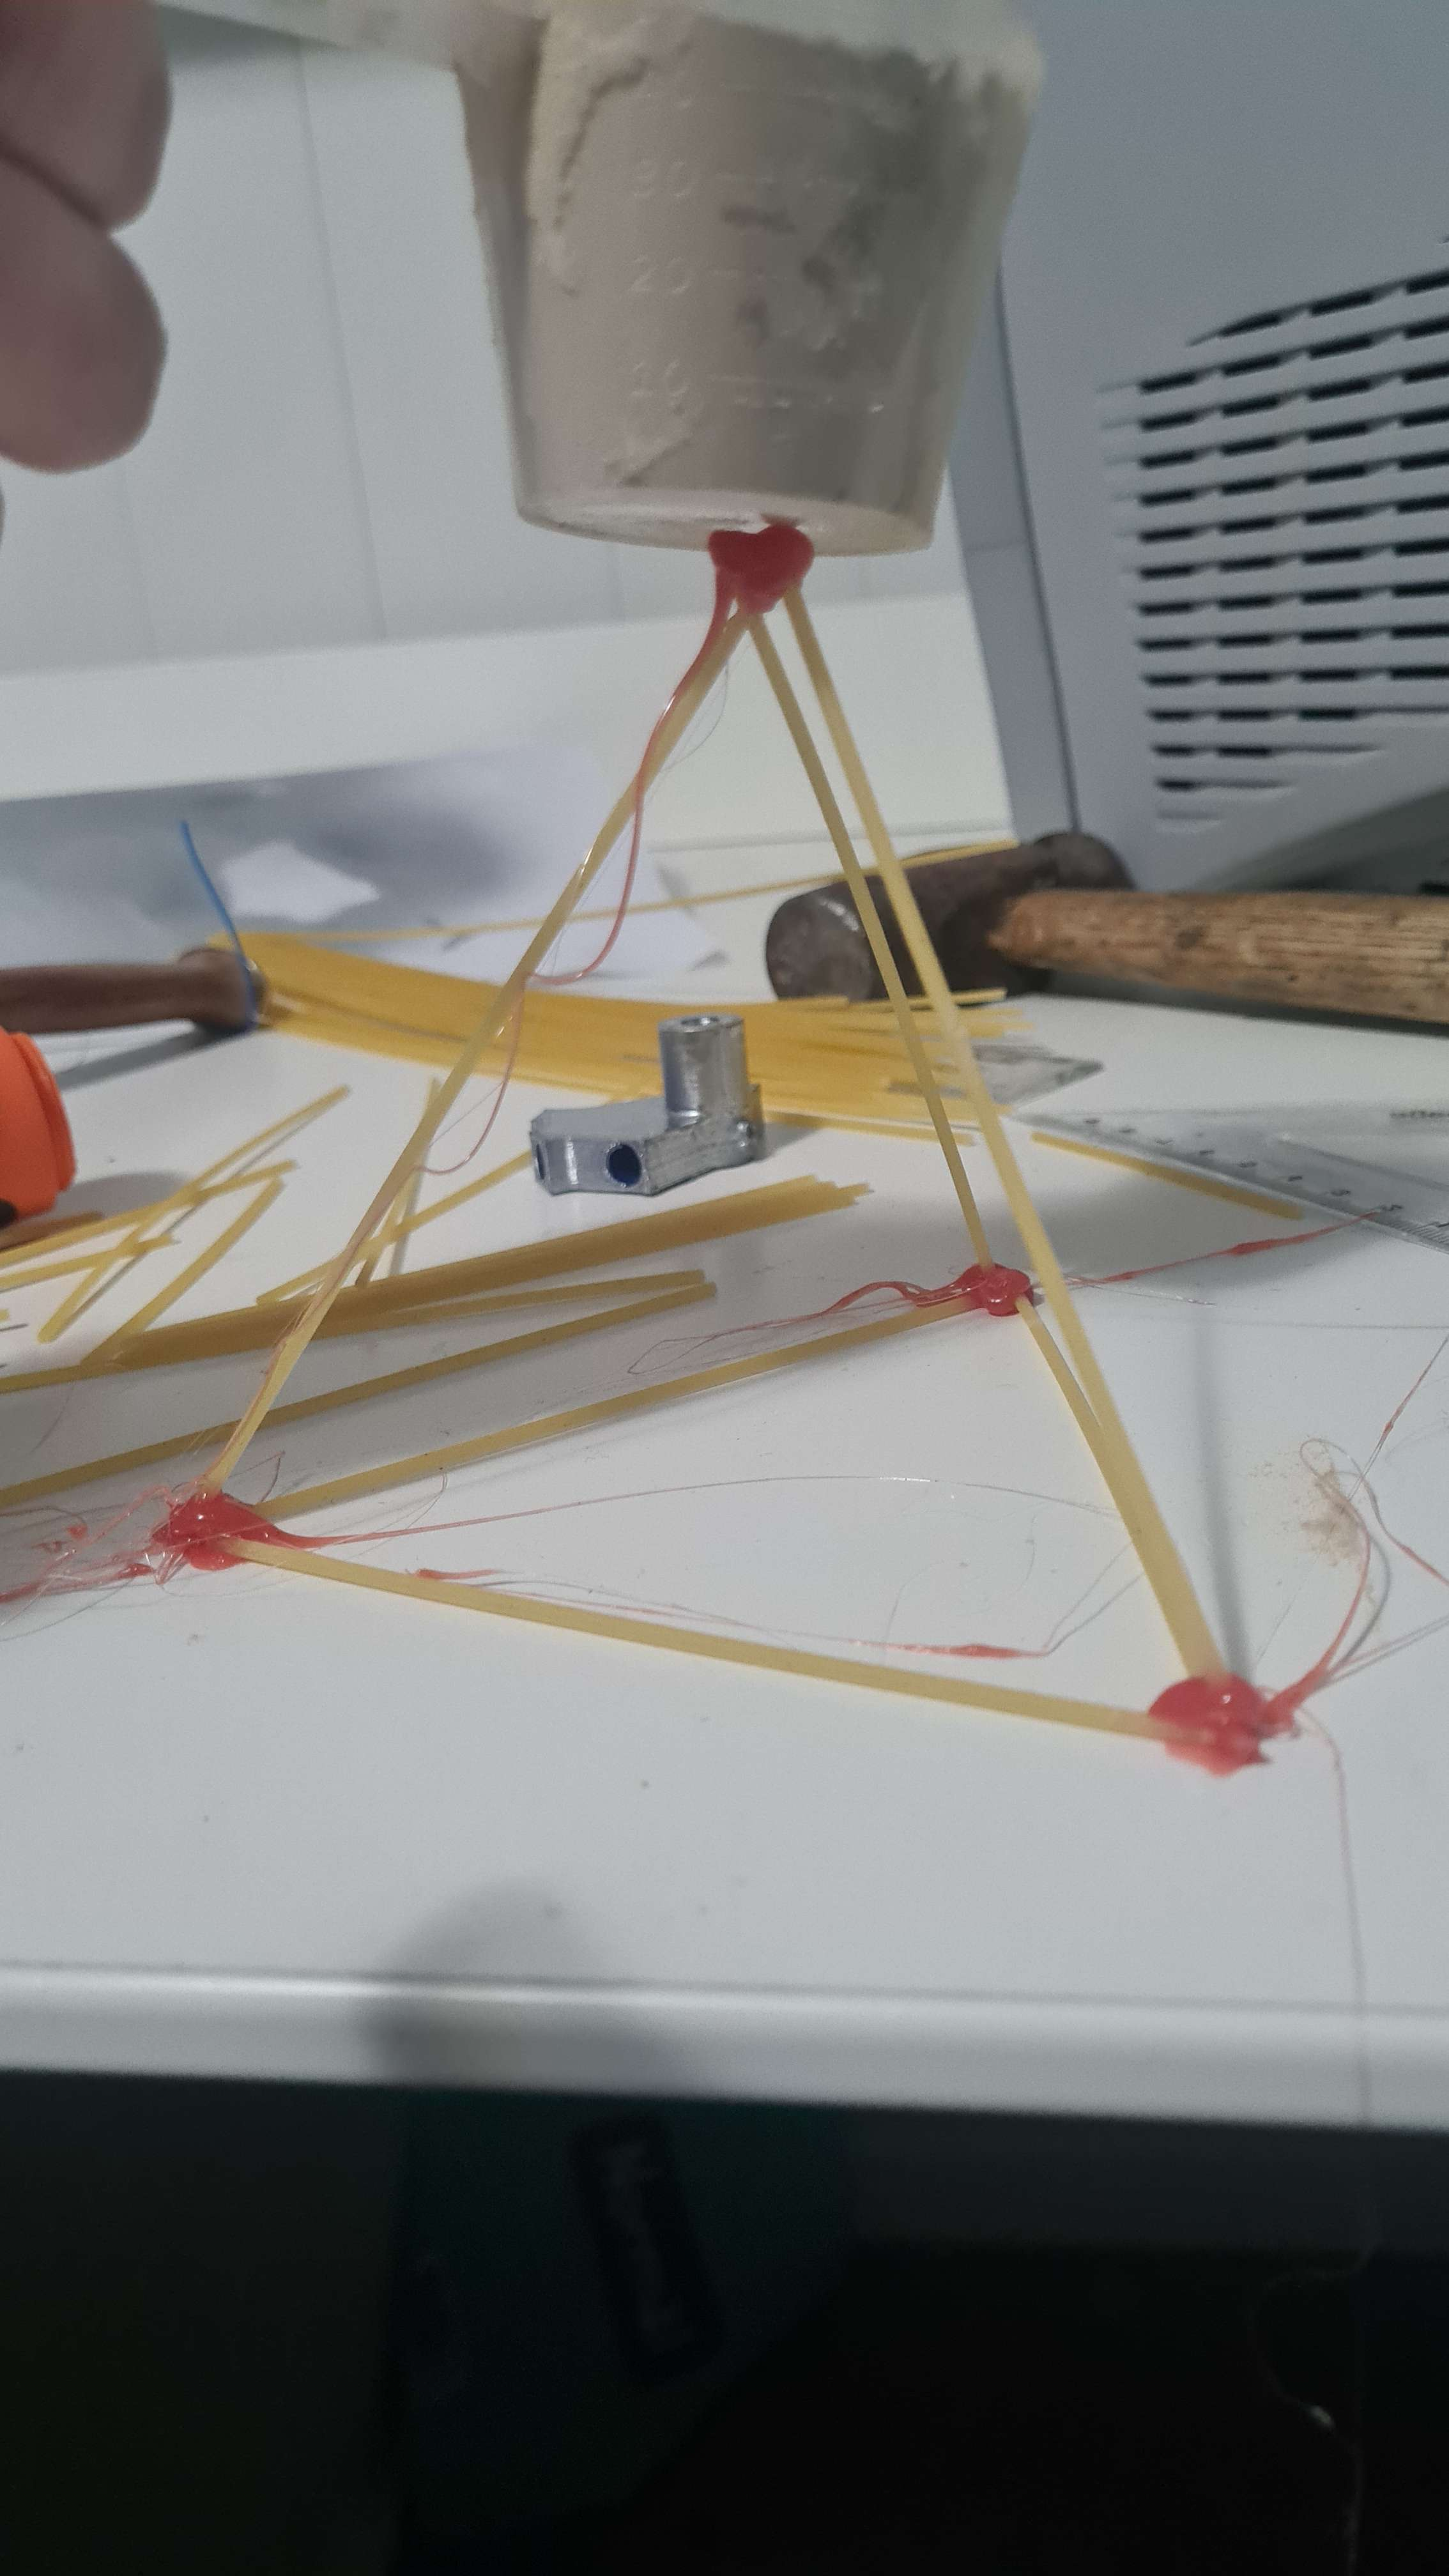
\includegraphics[width=\subimgw]{tetrehedra-a}
		\caption{Compression bucle isomorphism}

		\label{fig:tetrehedra:a}
	\end{subfigure}%
	\begin{subfigure}{.5\textwidth}
		\centering
		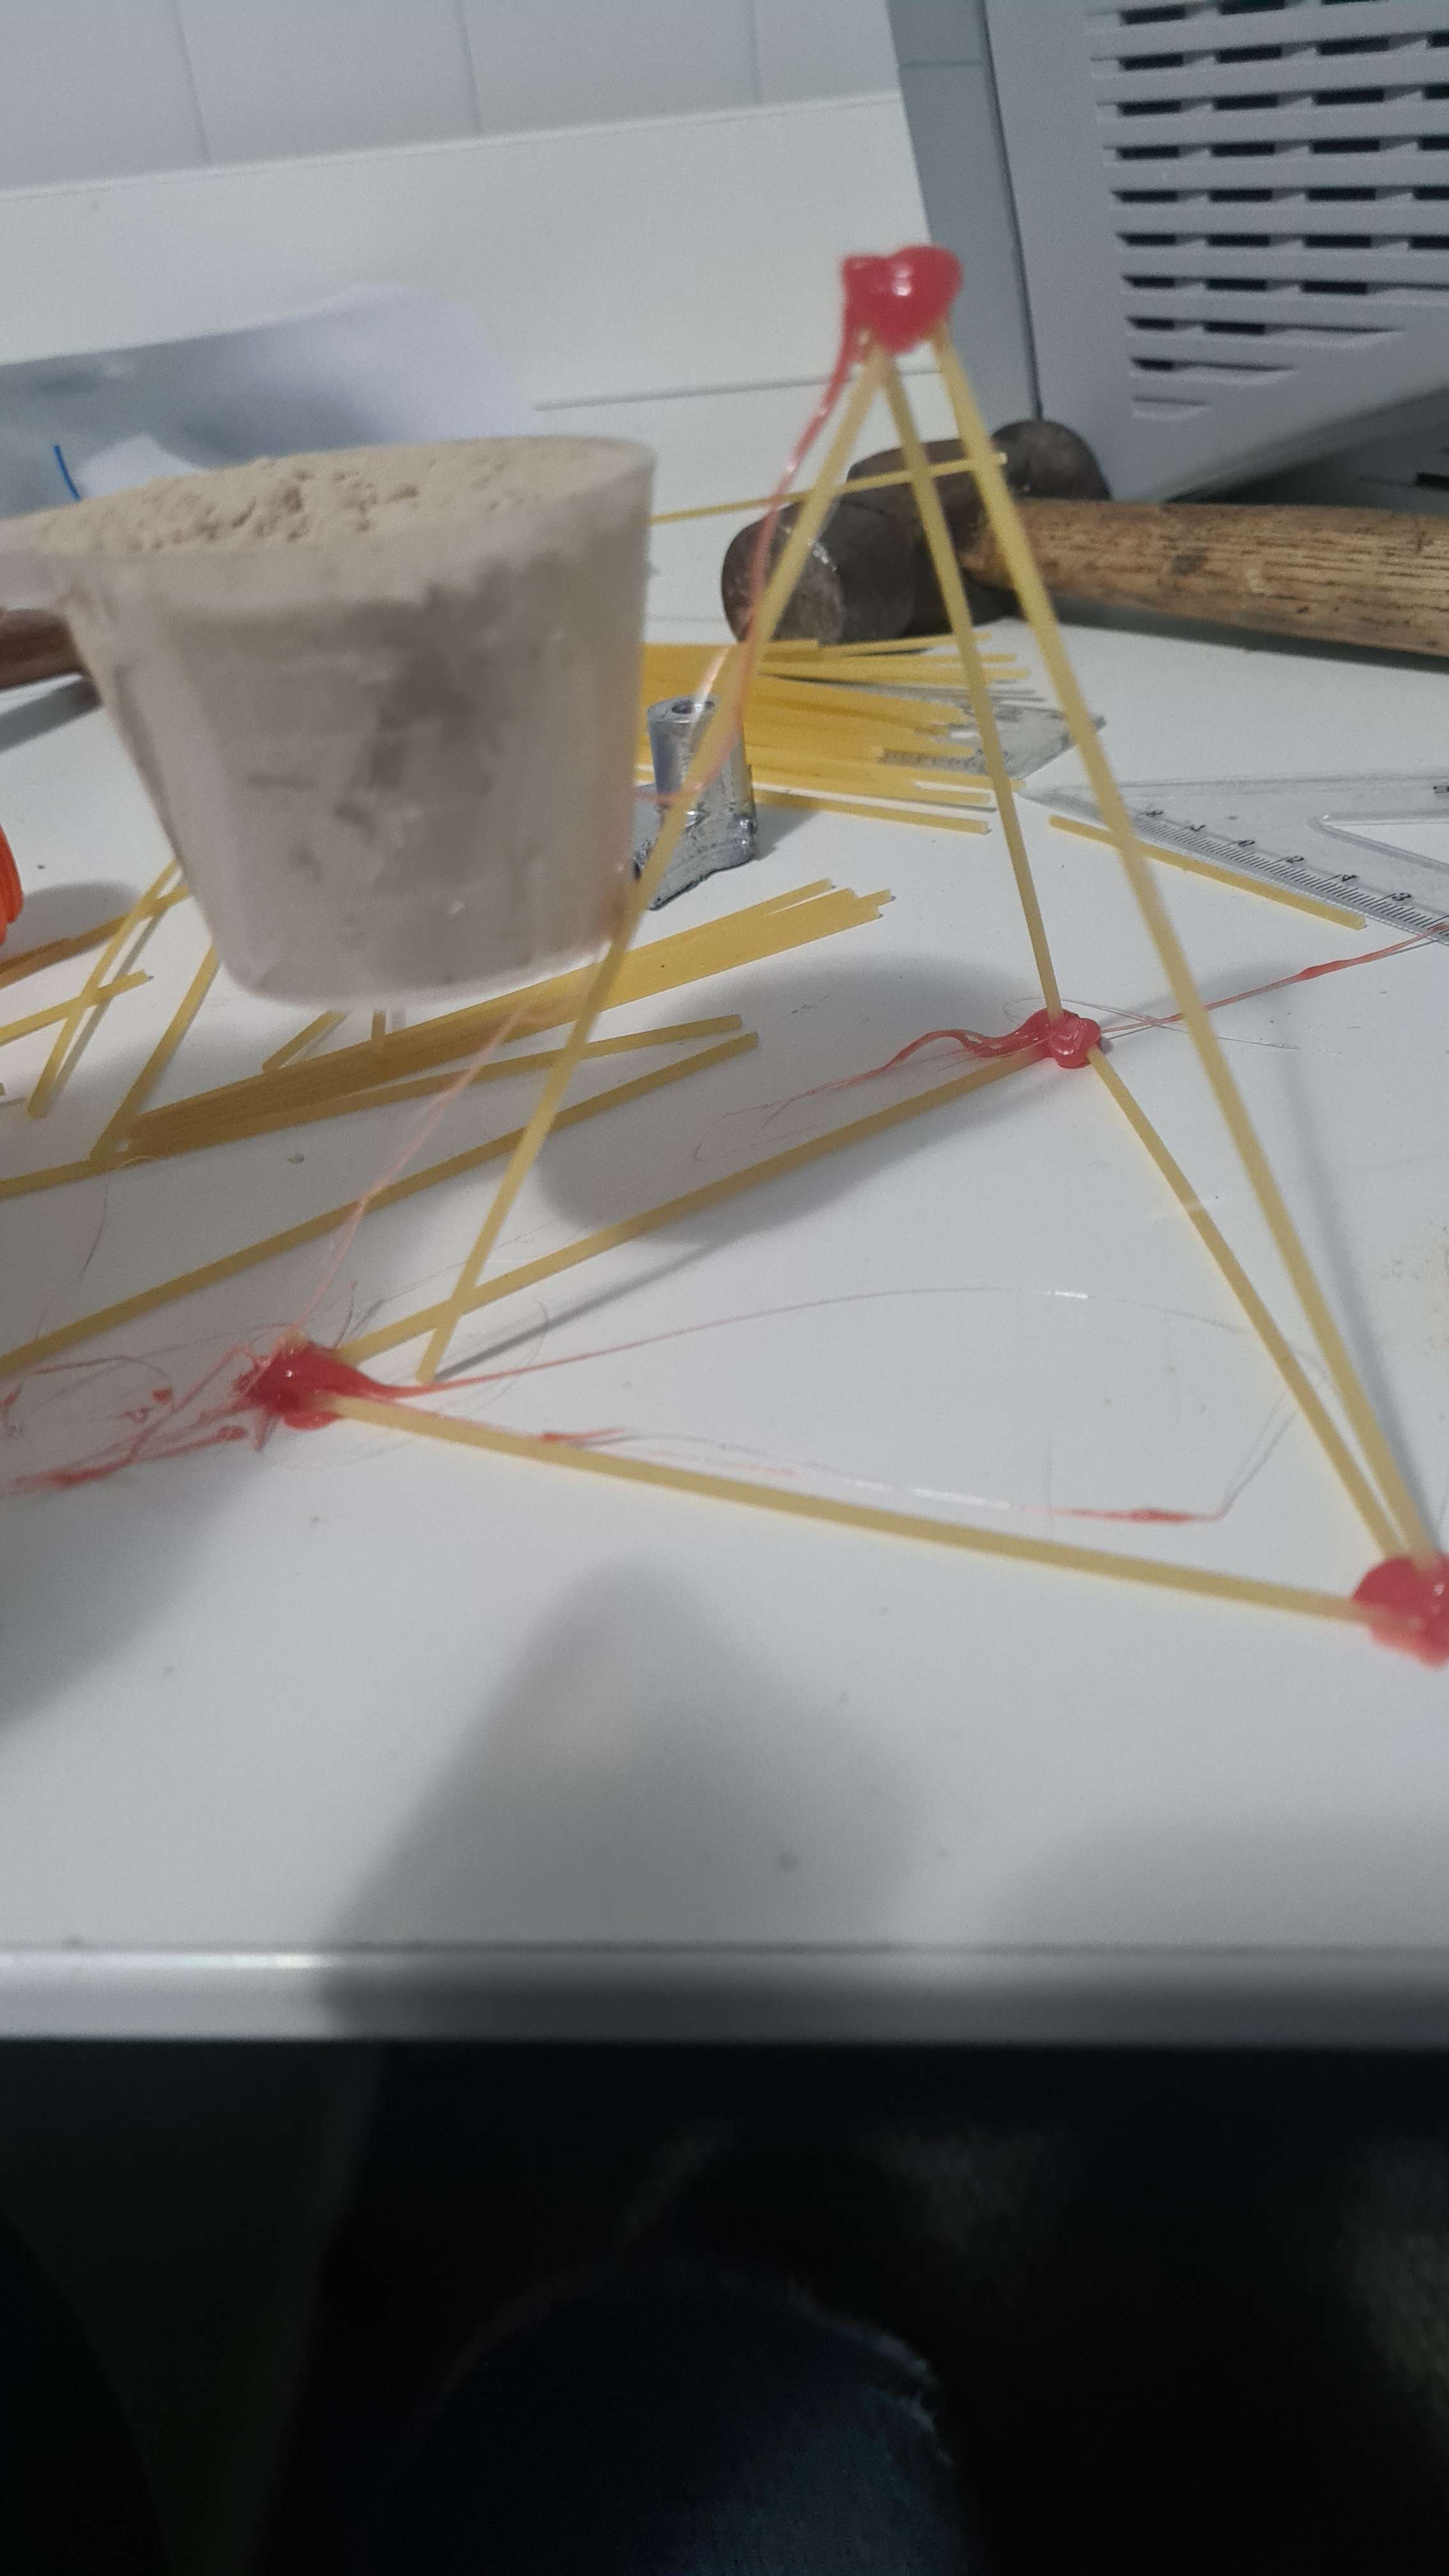
\includegraphics[width=\subimgw]{tetrehedra-b}
		\caption{Buckle force direction of tetrehedra}

		\label{fig:tetrehedra:untranslated}
	\end{subfigure}

	\caption{Tetrehedra}
	\label{fig:tetrehedra}
\end{figure}

Rektangulær trekant har de samme styrkene som en likebeint trekant hvor den korteste kateten tåler mest siden den fordeler kraften på de lengere katetene, men det dumme med rektangulær pyramide er at den kan oppleve planforskyving.

\begin{figure}[H]
	\begin{subfigure}{.5\textwidth}
		\centering
		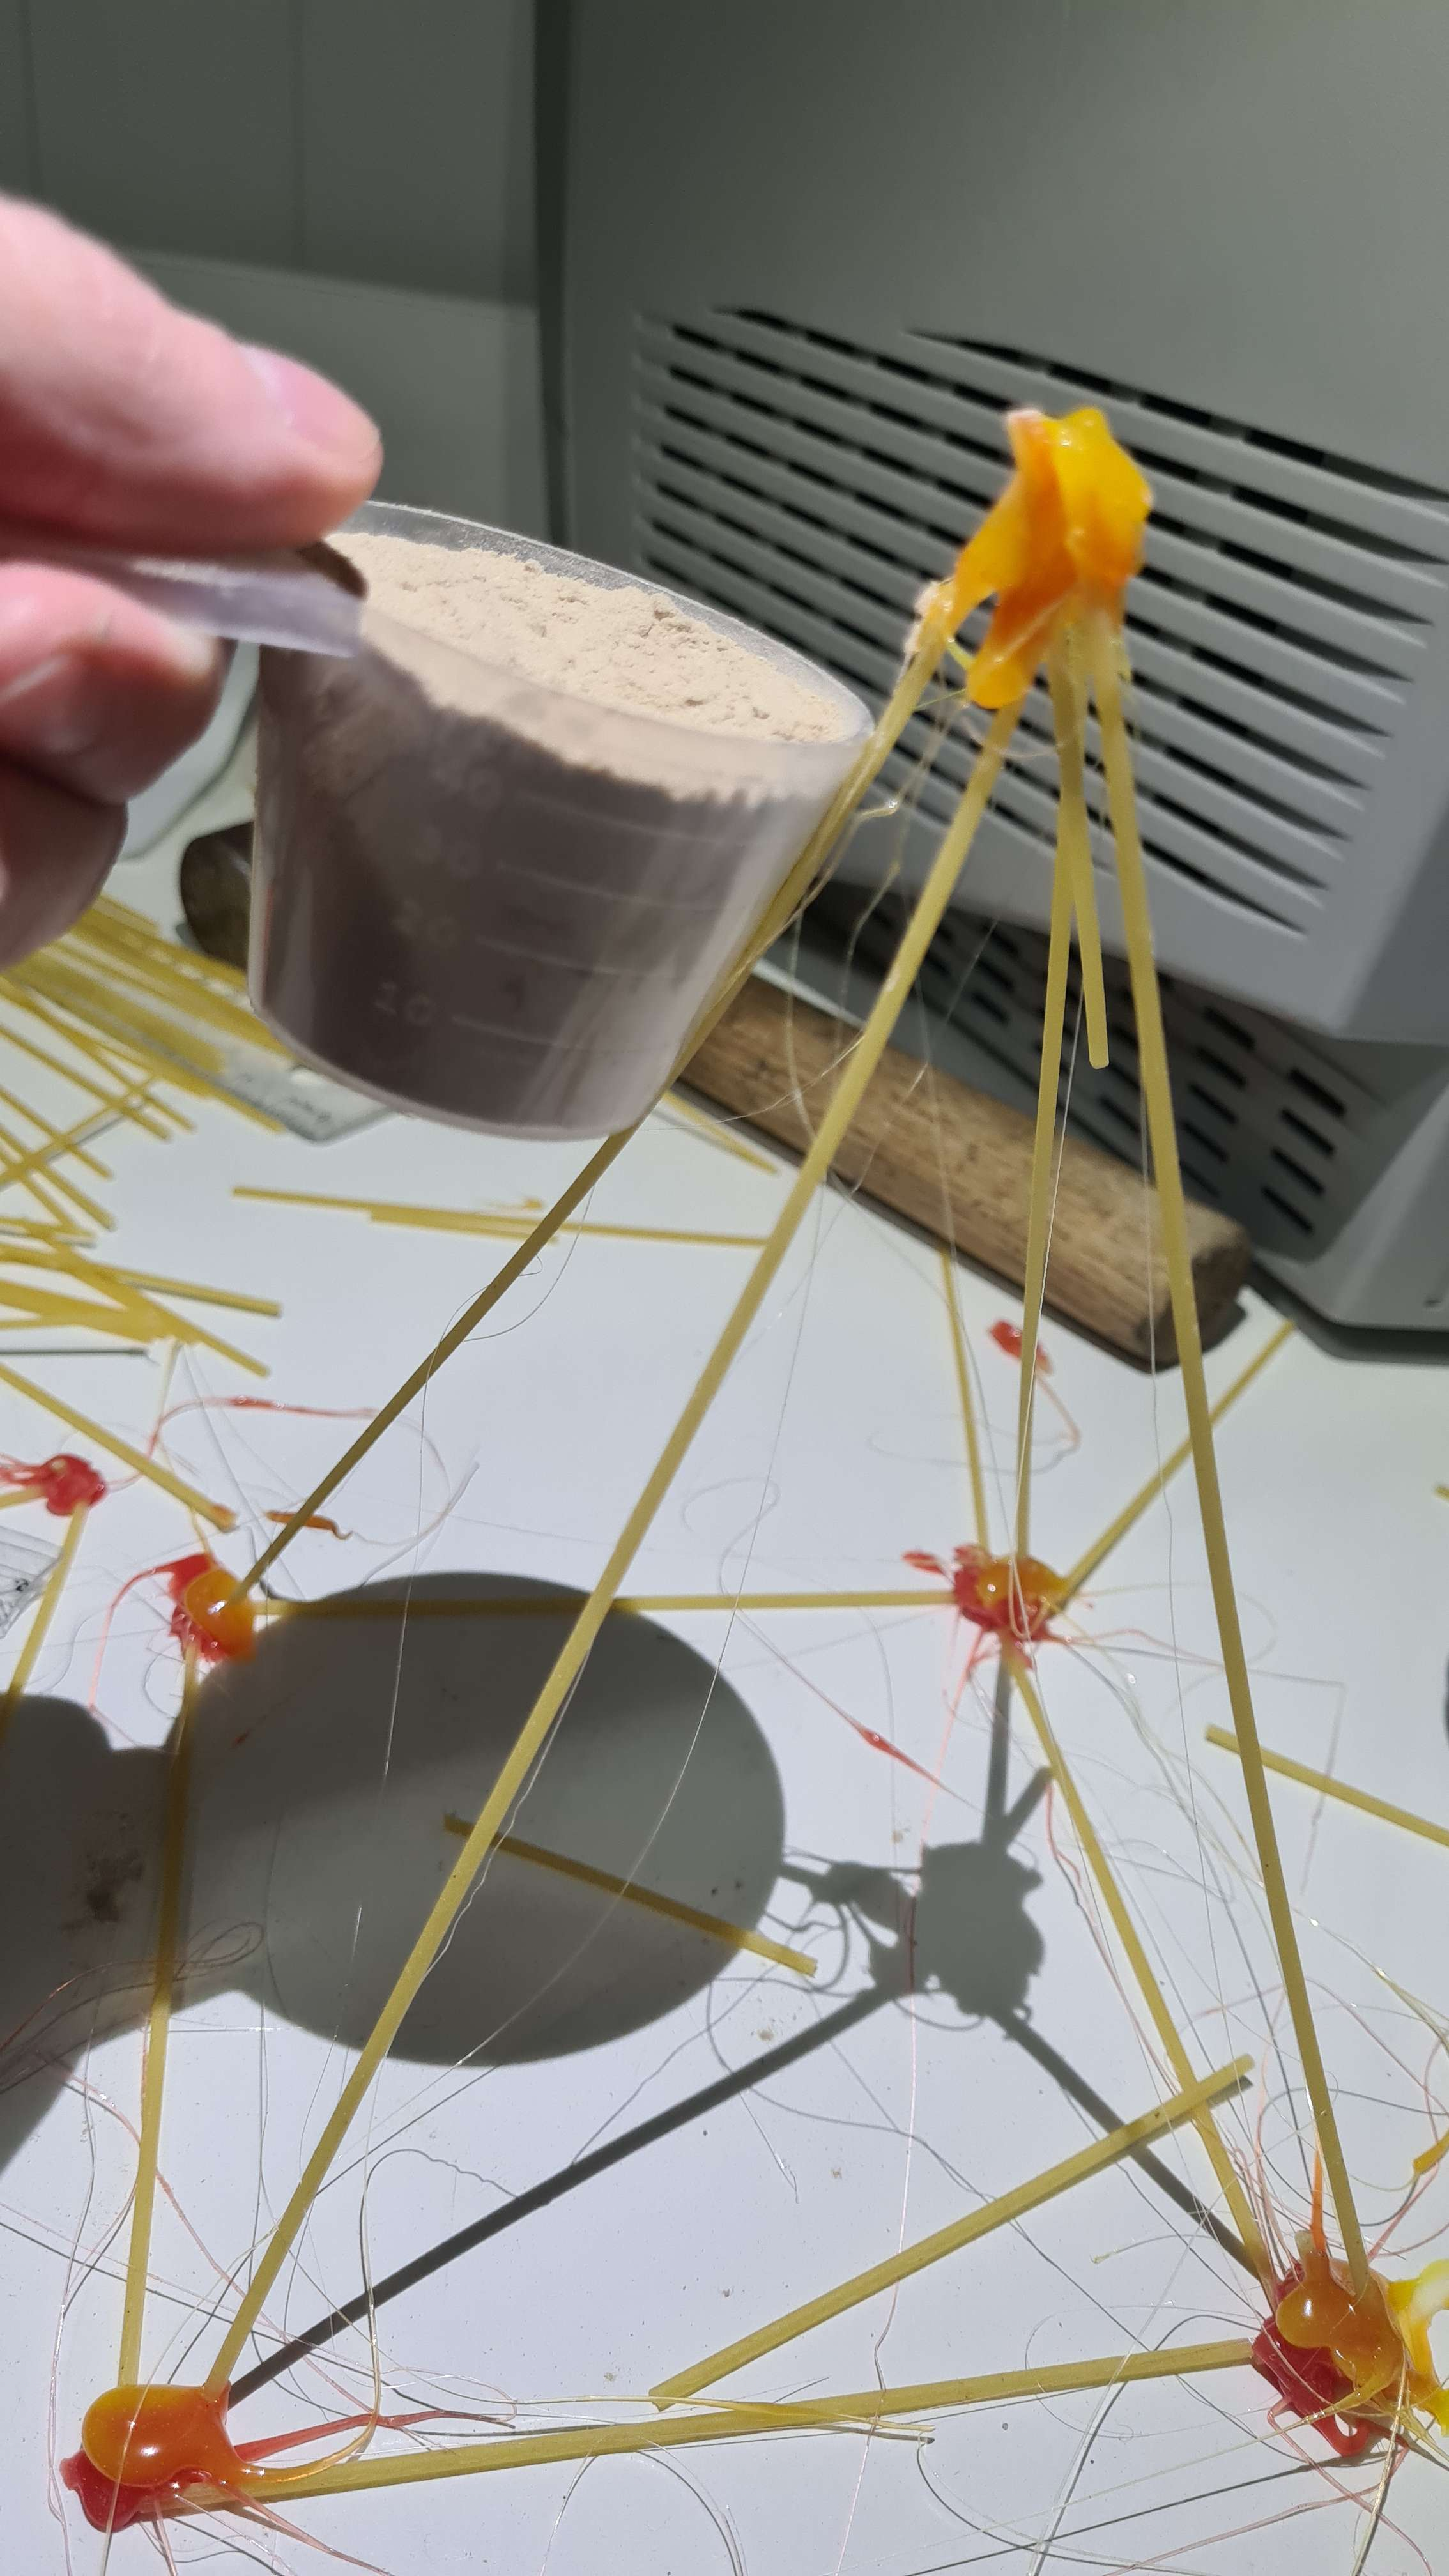
\includegraphics[width=\subimgw]{pyramid-a}

		\caption{Compression bucle of quad-pyramid}
		\label{fig:pyramid:a}
	\end{subfigure}%
	\begin{subfigure}{.5\textwidth}
		\centering
		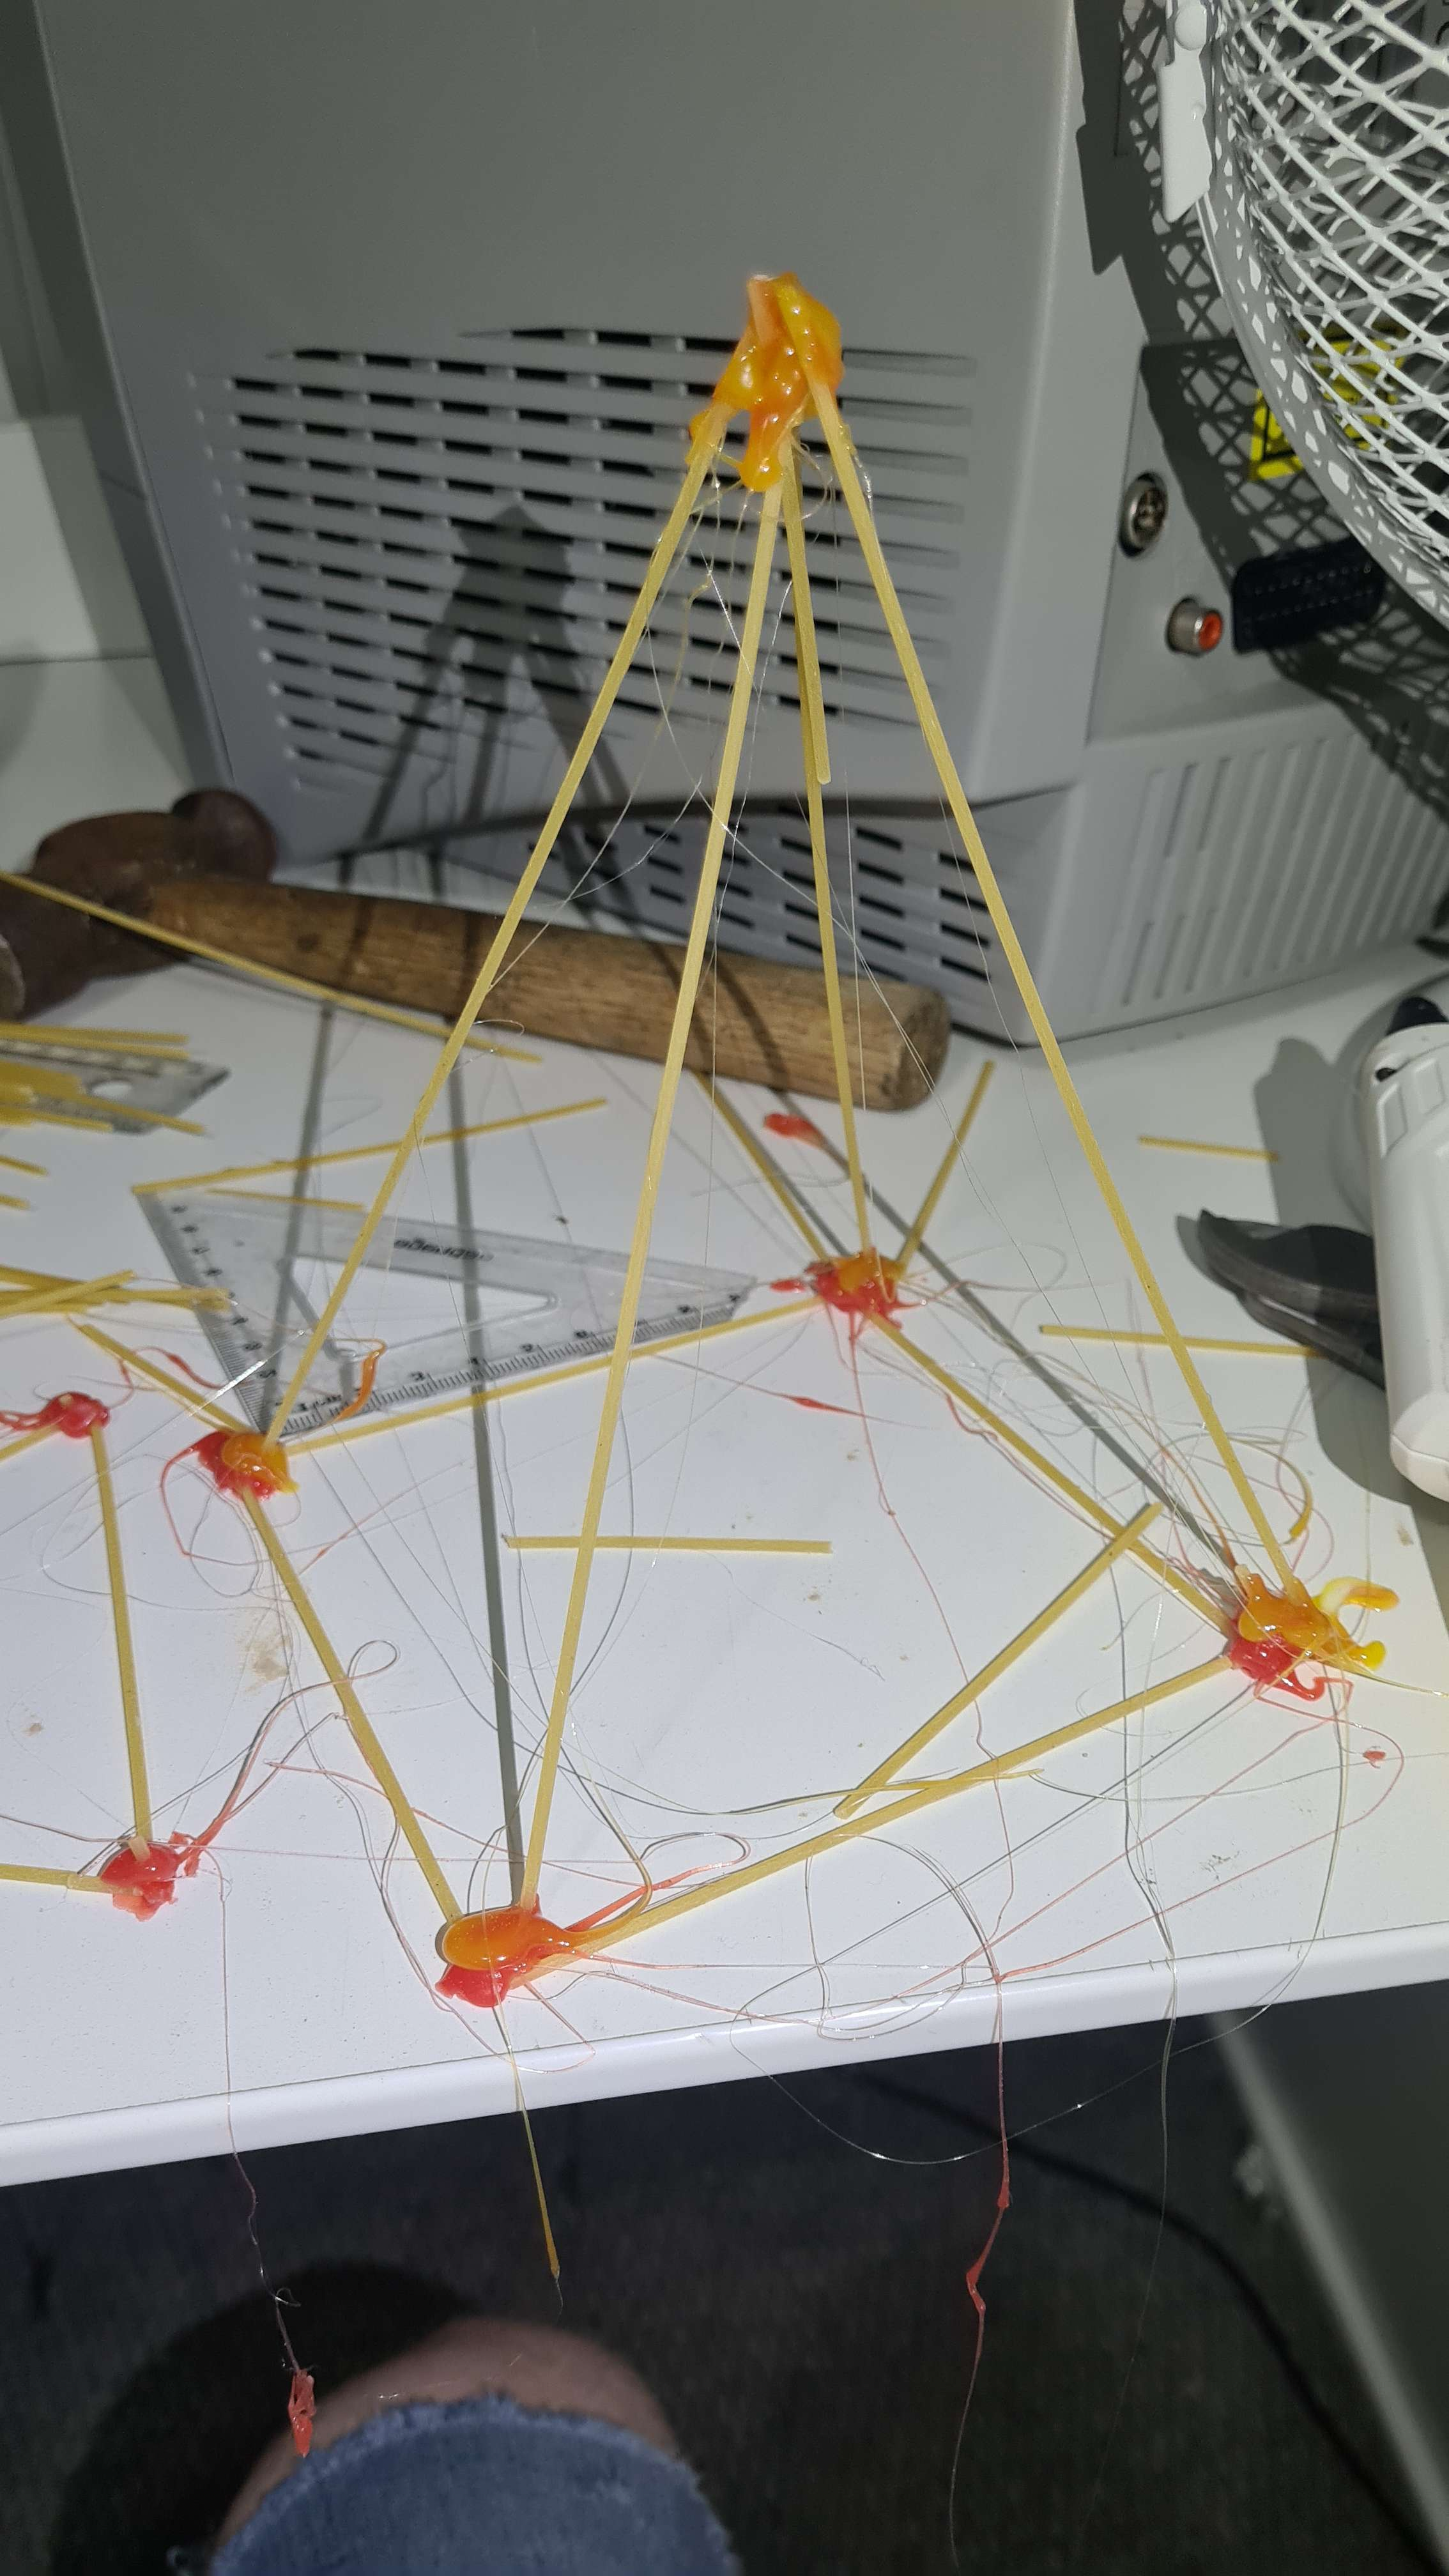
\includegraphics[width=\subimgw]{pyramid-untranslated}

		\caption{Buckle force direction of tetrehedra}
		\label{fig:pyramid:untranslated}
	\end{subfigure}

	\caption{Tetrehedra}
	\label{fig:pyramid}
\end{figure}

En kube er den svakeste formen siden den vil oppleve plan forskyving og knekke enkelt Figure \ref{fig:cube}

\begin{figure}[H]
	\begin{subfigure}{.5\textwidth}
		\centering
		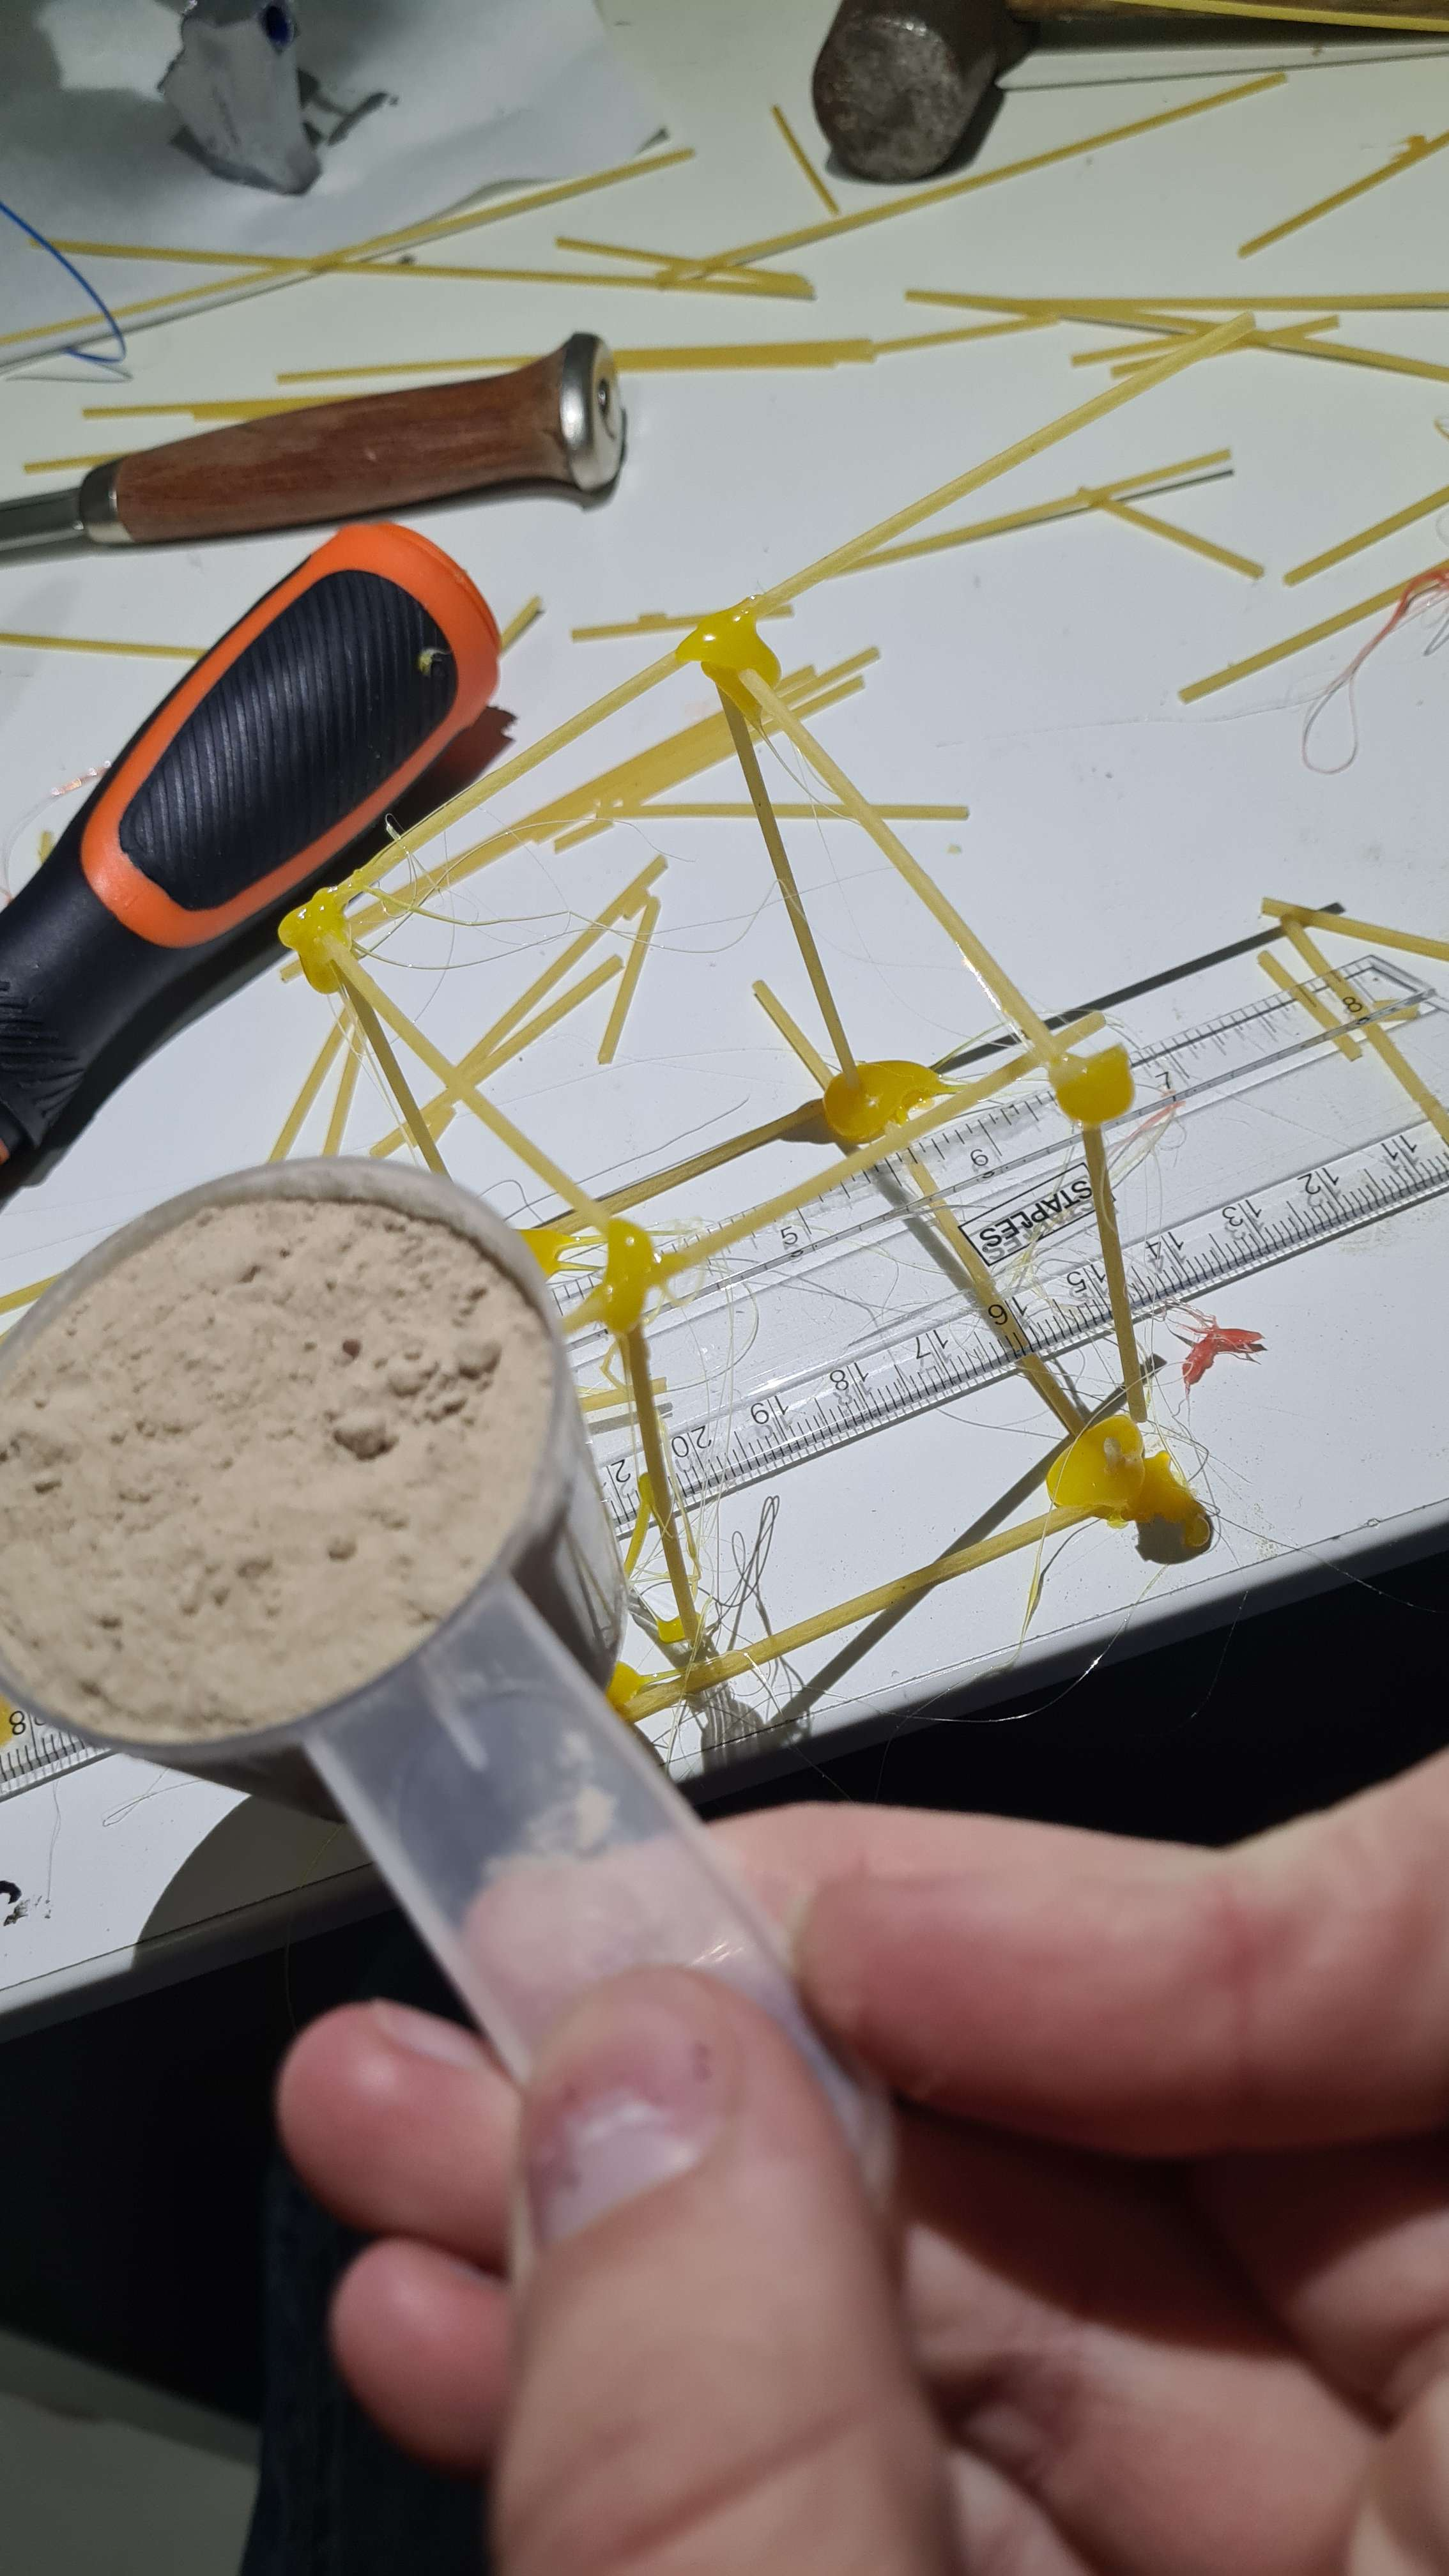
\includegraphics[width=\subimgw]{cube-a}

		\caption{Cube}
		\label{fig:cube:a}
	\end{subfigure}%
	\begin{subfigure}{.5\textwidth}
		\centering
		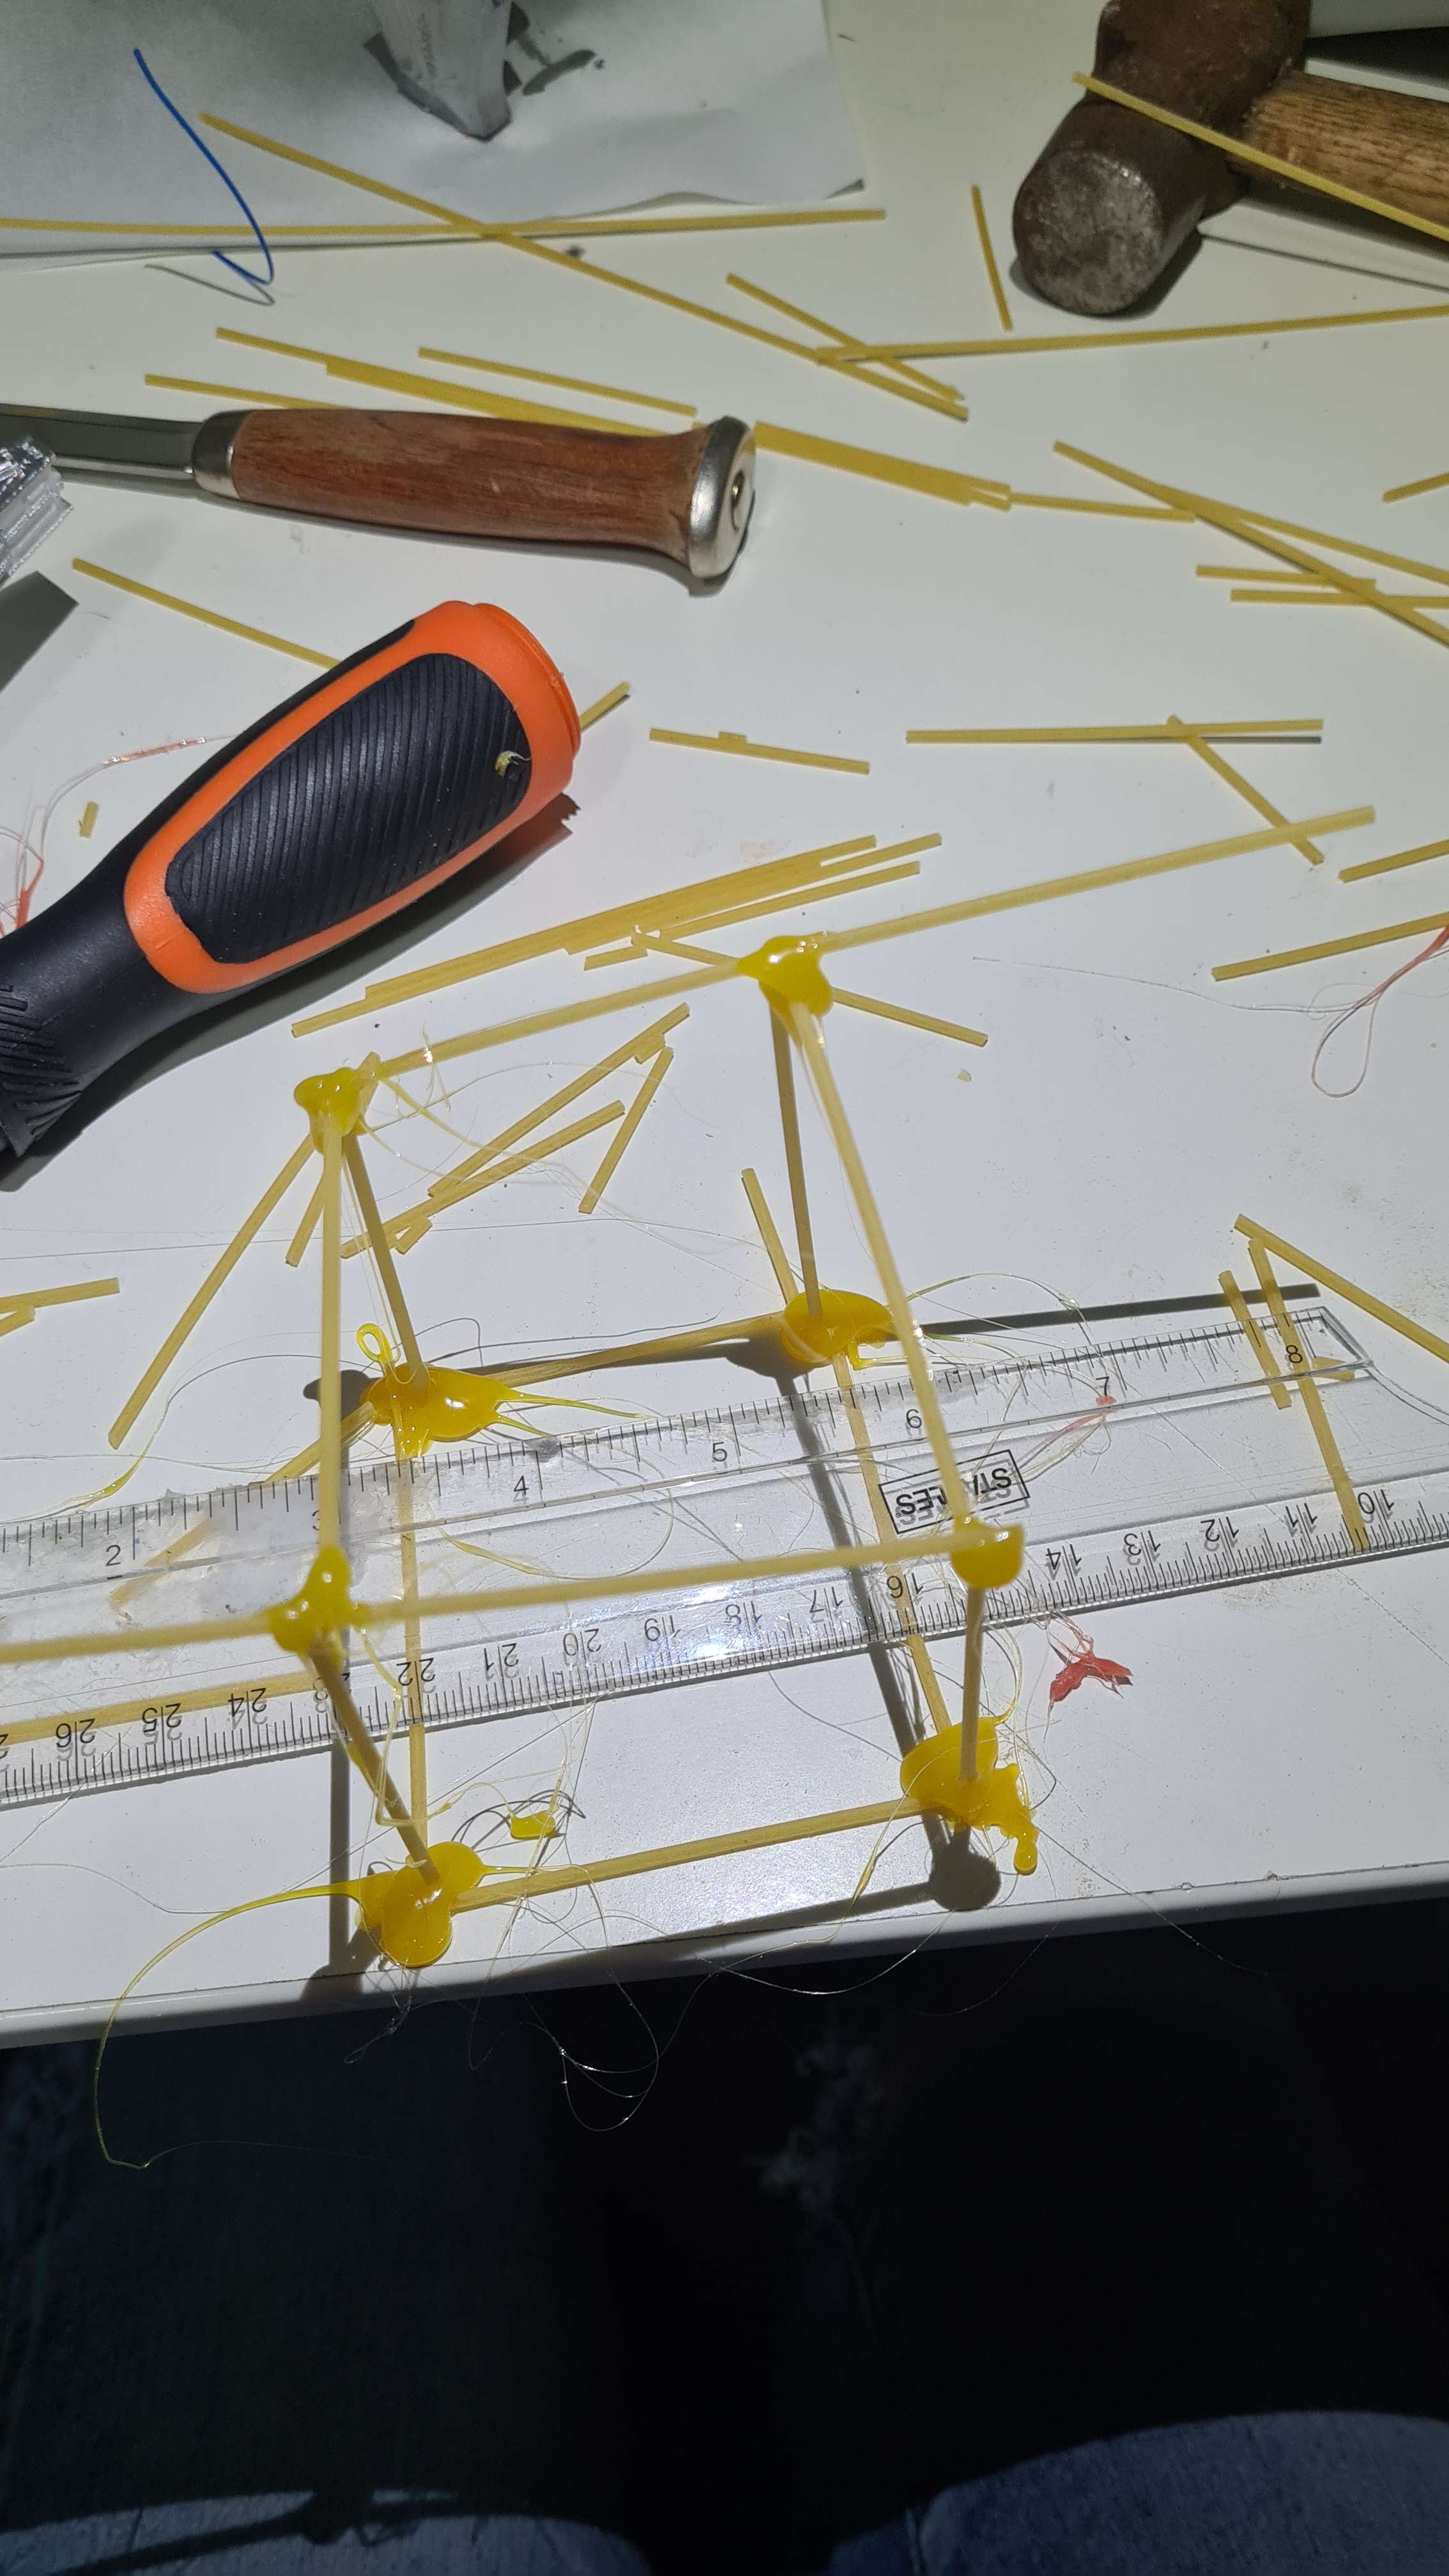
\includegraphics[width=\subimgw]{cube-untranslated}

		\caption{Undemonstartive cube}
		\label{fig:cube:untranslated}
	\end{subfigure}

	\caption{Cube}
	\label{fig:cube}
\end{figure}

\addcontentsline{toc}{section}{Oppgave 2}
\section*{Oppgave 2}

I denne oppgaven skulle man regne ut en målestokk for gruppens modellbru. Dette gjør mann med å bruke bruen virkelige størrelse og dele det på gruppens utvalgte målestokk

\addcontentsline{toc}{section}{Oppgave 3}
\section*{Oppgave 3}


\begin{figure}[t]
	\centering
	\includegraphics[width=.8\linewidth]{frame00000}

	\caption {OpenSCAD dump of bride including a legend of the different measurements.}
	\label{fig:bridge}
\end{figure}

I oppgave 3 skulle man bruke målestokken man har regnet ut tidligere for å lage en arbeidstegning. Dette skulle egentlig gjøres på ark som ble gjort, men når dette ble gjort var ikke tegningen nøyaktig og den ble heller programer inn i open SCAD for å få den mest mulig nøyaktig.

\addcontentsline{toc}{section}{Oppgave 4}
\section*{Oppgave 4}

\textbf {Lofoten}

Fisk: Lofoten er kjent rundt om i verden for sin fisker kultur. Derfor måtte vi intigrere deres kultur in i vårt bru design. Så det er 3d printed flere båter og fisker som kan festes på for å symbolisere dette.

Pride: Lofoten er blant de kommunene med høyest rate av mennesker som aksepterer homofile. Dette er også blant de kommunene som var først til å vie homofile med grunnlag på at dette var den kommunen med den første homofile presten og i dag er opp mot halvparten av prestene i kommunen homofil. dette er grunnen til at vår bru har et pride flag festet på seg

Miljø: det å bygge en bru er en prosess som krever mye energi og ressurser som er veldig skadelig for miljøet. Ifølge Architecture 2030 så står Bygg og konstruksjons industrien for 40\% av årlige utslipp dette er grunnen til at vår bru er bygget med sol celle panel slik at bruen etter mange vil bli karbon nøytral og i tillegg hjelpe lokal miljøet

\addcontentsline{toc}{section}{Oppgave 5}
\section*{Oppgave 5}

\addcontentsline{toc}{section}{Oppgave 6}
\section*{Oppgave 6}

\addcontentsline{toc}{section}{Oppgave 7}
\section*{Oppgave 7}

\chapter{Appendix}

\section{Refrence to OpenSCAD code}

\lstinputlisting{../bridge.scad}

\section{Recrence to Python JHU-generation code}

\lstinputlisting[language=Python]{../jhu-gen.py}

\addcontentsline{toc}{section}{List of figures}
\listoffigures

\end{document}

